\documentclass[a4paper, 14pt, fleqn]{extarticle}
\usepackage[russian]{babel}
\usepackage{enumitem}
\usepackage{fefutitle}
\usepackage{xcolor}
\usepackage{amsmath}
\usepackage{amssymb}
\usepackage{graphicx}
\usepackage[justification=centering]{caption}
\usepackage{float}
\usepackage[T2A]{fontenc}
\usepackage[utf8x]{inputenc}
\usepackage{pythonlisting}
\usepackage{listingsutf8}
\usepackage{ucs}
\usepackage{mathtext}
\usepackage{upgreek}
\usepackage{textcomp}
\usepackage{amsfonts}
\usepackage{mathtools}
\usepackage{xstring}
\usepackage{changepage}
\usepackage{makecell}
\usepackage{longtable}

\begin{document}
	
	\pagebreak
	\parskip = 5pt

	\section{Численное решение задачи Коши}
		\subsection{Постановка задачи}
			\noindent Необходимо решить задачу Коши ($x \in [0;2]$):
			\begin{equation*}
				\begin{cases}
					y'=\cos{\bigg(\dfrac{5}{2}x - \dfrac{1}{2}y \bigg) }
					\\
					y(0)=0
				\end{cases}
			\end{equation*}
		
			Решение выполнить тремя методами: Эйлера, улучшенный метод Эйлера и Рунге-Кутта 4-го порядка. Сравнить результаты.
	
		\subsection{Решение}
		
			\subsubsection{Аналитическое решение}
			
				\[y'=\cos{\bigg(\dfrac{5}{2}x - \dfrac{1}{2}y \bigg) }\]
				Характеристика: линейное неоднородное уравнение.
				
				Решение:
				\[ \arctan{\bigg(\dfrac{\sqrt{3}}{2} \tan{\dfrac{5x-y}{4}}\bigg)} = \dfrac{\sqrt{6}}{2}x + C \]
				Решение задачи Коши:
				\[y = 5x - 4\arctan{\bigg(\dfrac{2}{\sqrt{3}} \tan{\dfrac{\sqrt{6}}{2}x}\bigg)}\]
			
			\subsubsection{Метод Эйлера}
			
				Расчетная формула метода Эйлера:
				\begin{multline} 
					y_{i+1}=y_i+h*f(x_i,y_i), \text{ где } i=0,1...n;y'=f(x,y)
				\end{multline}
				
				Решение реализовано с помощью программы \textit{Python}. Результаты программы представлены в таблице, где $y^*_i$ -- точное решение, а $y_i$ -- приближенное:
				
				\begin{figure}[h]
					\centering
					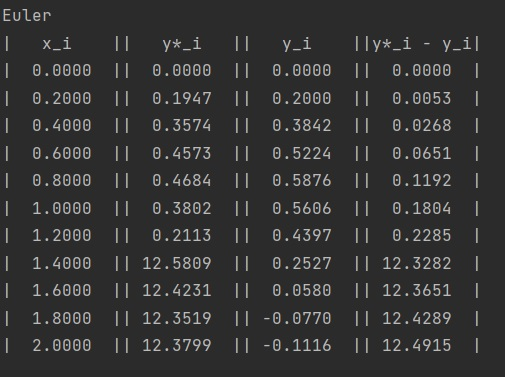
\includegraphics[width = 0.6\linewidth]{1.jpg}
				\end{figure}
				
				\begin{figure}[h]
					\centering
					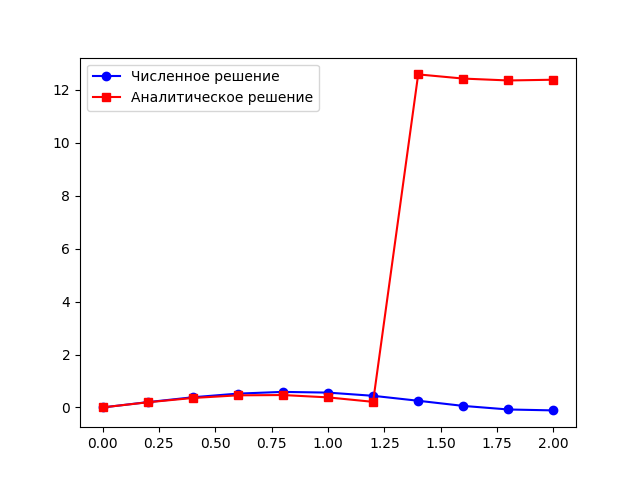
\includegraphics[width = 0.6\linewidth]{euler.png}
					\caption{График точного решения и решения методом Эйлера}
				\end{figure}
				\pagebreak
				
			    \begin{figure}[h]
			    	\centering
			    	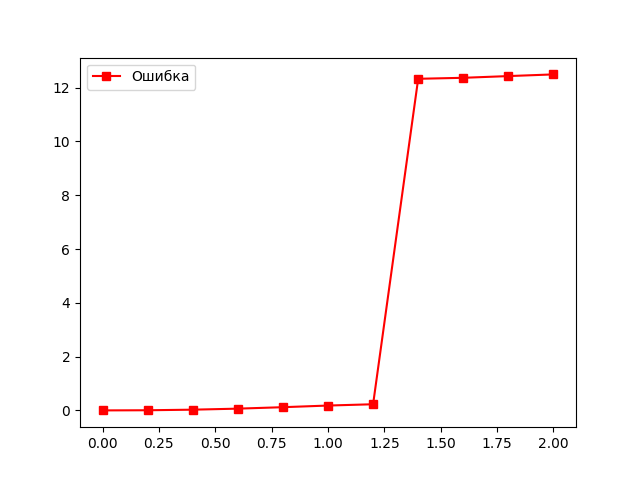
\includegraphics[width = 0.6\linewidth]{euler-error.png}
			    	\caption{График ошибки}
			    \end{figure}
			
			\pagebreak
			\subsubsection{Улучшенный метод Эйлера}
			
				Расчетная формула улучшенного метода Эйлера:
				\begin{multline} 
					y_{i+1}=y_i+\dfrac{h}{2}(f(x_i,y_i)+f(x_{i+1},y*_{i+1})), \text{ где } i=0,1...n;\\y*_{i+1}\text{ -- значение в классическом методе Эйлера}
				\end{multline}
				
				Решение реализовано с помощью программы \textit{Python}. Результаты программы представлены в таблице, где $y^*_i$ -- точное решение, а $y_i$ -- приближенное:
				\begin{figure}[h]
					\centering
					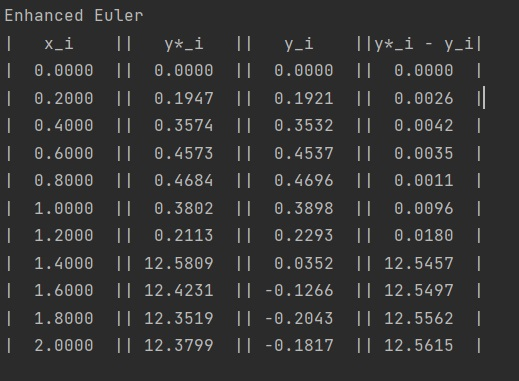
\includegraphics[width = 0.6\linewidth]{2.jpg}
				\end{figure}
				\pagebreak
				\begin{figure}[h]
					\centering
					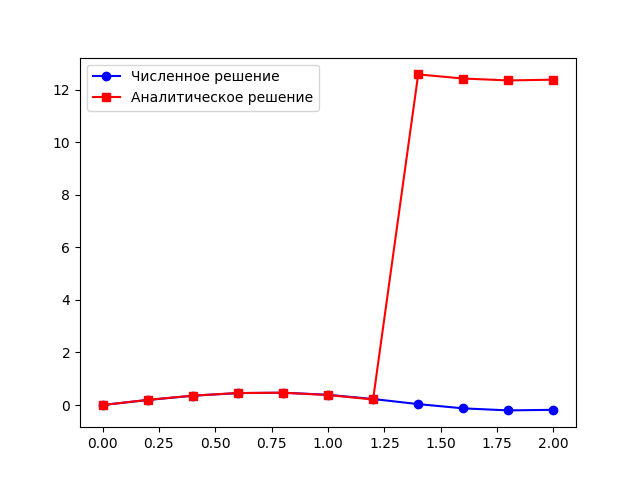
\includegraphics[width = 0.6\linewidth]{euler-enhanced.png}
					\caption{График точного решения и решения улучшенным методом Эйлера}
				\end{figure}
				\begin{figure}[h]
					\centering
					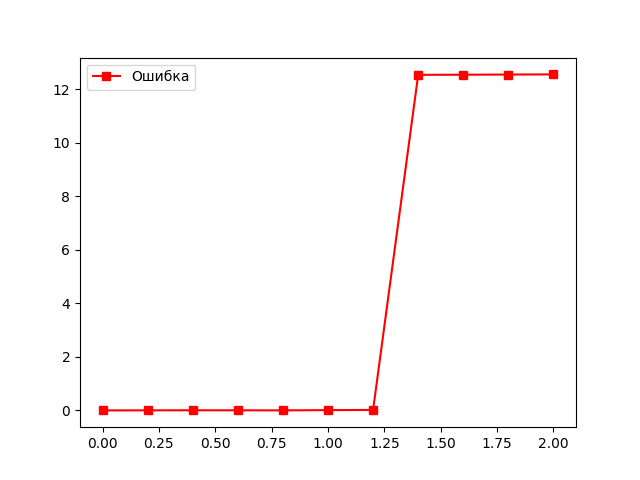
\includegraphics[width = 0.6\linewidth]{euler-enhanced-error.png}
					\caption{График ошибки}
				\end{figure}
			\pagebreak
				
			\subsubsection{Метод Рунге-Кутта 4-го порядка}
			
				Расчетная формула метода Рунге-Кутта 4-го порядка:
				\begin{multline}
					y_{i+1}=y_{i}+(k_1+2*k_2+2*k_3+k_4)/6 \\
					k_1=h*f(x_i,y_i)\\
					k_2=h*f(x_i+h/2,y_i+h*k_1/2)\\ 
					k_3=h*f(x_i+h/2,y_i+h*k_2/2)\\
					k_4=h*f(x_i+h,y_i+h*k_3)\\
				\end{multline}
				
				Решение реализовано с помощью программы \textit{Python}. Результаты программы представлены в таблице, где $y^*_i$ -- точное решение, а $y_i$ -- приближенное:
				
				\begin{figure}[h]
					\centering
					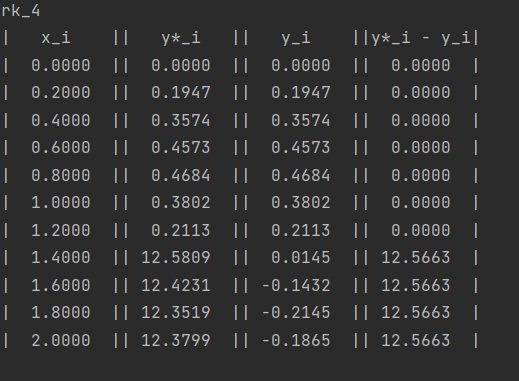
\includegraphics[width = 0.6\linewidth]{3.jpg}
				\end{figure}
			\pagebreak
			
				\begin{figure}[h]
					\centering
					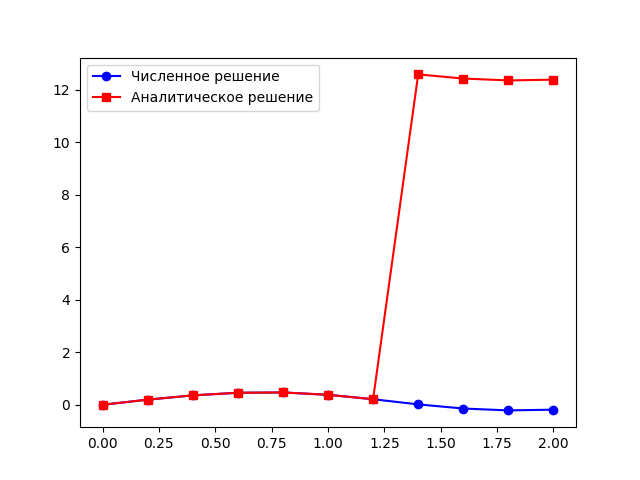
\includegraphics[width = 0.6\linewidth]{rk4.png}
					\caption{График точного решения и решения методом Рунге-Кутта 4-го порядка}
				\end{figure}
			
				\begin{figure}[h]
					\centering
					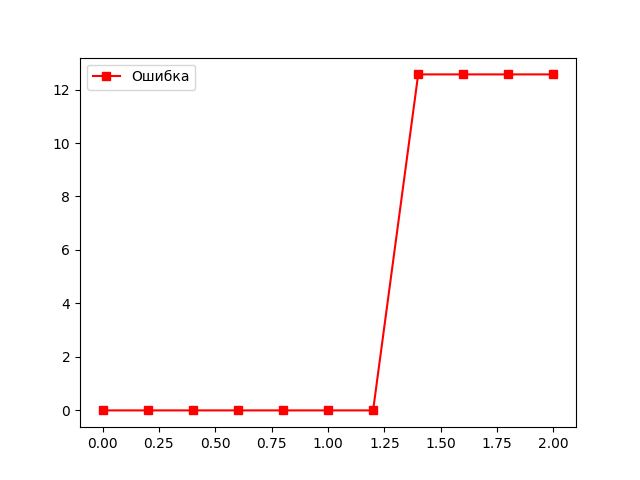
\includegraphics[width = 0.6\linewidth]{rk4-error.png}
					\caption{График ошибки}
				\end{figure}
			
	\pagebreak
	
	\section{Заключение}
	
		\begin{figure}[h]
			\centering
			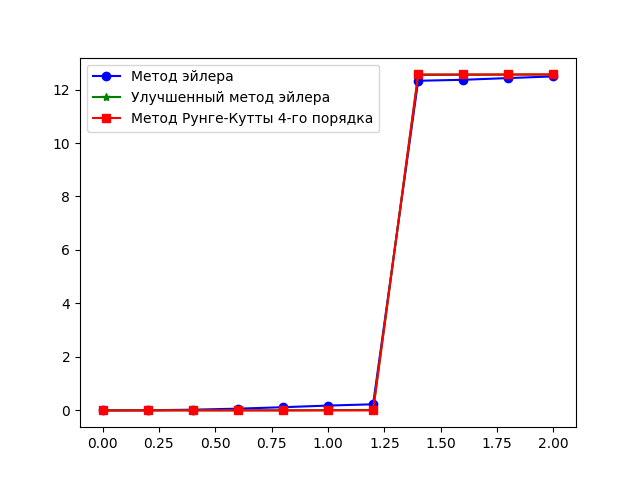
\includegraphics[width = 0.9\linewidth]{error-union.png}
		\end{figure}
	
		На интервале [0, 1] метод Рунге-Кутты 4-го порядка показал самую лучшую точность. Далее идет модифицированный метод Эйлера. На последнем месте по точности оказался метод Эйлера. На интервале [1, 2] аналитическое решение имеет складку, ни один из методов не смог ее воспроизвести.
	\pagebreak
	\section{Код}
	
	\lstinputlisting[language=Python]{./main.py}
	
\end{document}	